\let\negmedspace\undefined
\let\negthickspace\undefined
\documentclass[journal,12pt,onecolumn]{IEEEtran}
\usepackage{cite}
\usepackage{amsmath,amssymb,amsfonts,amsthm}
\usepackage{algorithmic}
\usepackage{graphicx}
\graphicspath{{Figs/}}
\usepackage{textcomp}
\usepackage{xcolor}
\usepackage{txfonts}
\usepackage{listings}
\usepackage{enumitem}
\usepackage{mathtools}
\usepackage{gensymb}
\usepackage{comment}
\usepackage{caption}
\usepackage[breaklinks=true]{hyperref}
\usepackage{tkz-euclide} 
\usepackage{listings}
\usepackage{gvv}                                        
%\def\inputGnumericTable{}                                 
\usepackage[latin1]{inputenc}     
\usepackage{xparse}
\usepackage{color}                                            
\usepackage{array}                                            
\usepackage{longtable}                                       
\usepackage{calc}                                             
\usepackage{multirow}
\usepackage{multicol}
\usepackage{hhline}                                           
\usepackage{ifthen}                                           
\usepackage{lscape}
\usepackage{tabularx}
\usepackage{array}
\usepackage{float}
%\newtheorem{theorem}{Theorem}[section]
%\newtheorem{theorem}{Theorem}[section]
%\newtheorem{problem}{Problem}
%\newtheorem{proposition}{Proposition}[section]
%\newtheorem{lemma}{Lemma}[section]
%\newtheorem{corollary}[theorem]{Corollary}
%\newtheorem{example}{Example}[section]
%\newtheorem{definition}[problem]{Definition}

\begin{document}

\title{9.2.35}
\author{AI25BTECH11002 - Ayush Sunil Labhade}
\maketitle
%\renewcommand{\thefigure}{\theenumi}
%\renewcommand{\thetable}{\theenumi}

\textbf{Question :} Sketch the region \brak{x, 0} : y = $\sqrt{4 - x^2}$ and x-axis. Find the area of the region using integration.

\textbf{Solution :}

\begin{table}[h!]
  \centering
  \begin{tabular}{|l|l|}
  \hline
  Name & Value \\
  \hline
  Circle & $\vec{x}^\top\vec{x} - 4 = 0$ \\
  Line & $\vec{x} = \myvec{0\\0} + \kappa \myvec{1\\0}$ \\
  \hline
  \end{tabular}
  \caption*{Table : Circle}
  \label{9.2.35}
\end{table}

The parameters for the circle are :

\begin{align}
  \vec{V} &= \vec{I} & \vec{u} &= \vec{0} & f &= -4 
\end{align}

The parameters for the line are :

\begin{align}
  \vec{h} &= \myvec{0\\0} & \vec{m} &= \myvec{1\\0}
\end{align}

Substituting these in the below equation to find the intersection points :

\begin{align}
\kappa_i
	&= \frac{1}{\vec{m}^\top \vec{V}\vec{m}} \brak{
       -\,\vec{m}^\top\big(\vec{V}\vec{h}+\vec{u}\big)
       \;\pm\;
       \sqrt{ \big[\vec{m}^\top(\vec{V}\vec{h}+\vec{u})\big]^2
	- g(\vec{h})\,\big(\vec{m}^\top \vec{V}\vec{m}\big)}}\\
    g(\vec{x}) &= \vec{x}^\top\vec{x} - 4 \\
    g(\vec{h}) &= \vec{h}^\top\vec{h} - 4 \\
\kappa_i &= 
       -\,\vec{m}^\top\vec{h}
       \;\pm\;
       \sqrt{4 -\vec{h}^\top\vec{h}} \\
  \kappa_i &= 2,-2
\end{align}

Therefore the points of intersection are :

\begin{align}
  \vec{P_1} &= \myvec{2\\0} & \vec{P_2} &= \myvec{-2\\0}
\end{align}

Thus the area of the region is :

\begin{align}
  2 \int\limits_{0}^{2}\! \sqrt{4 - x^2}\, dx &= 2\pi
\end{align}

\pagebreak

\begin{figure}[H]
  \centering
  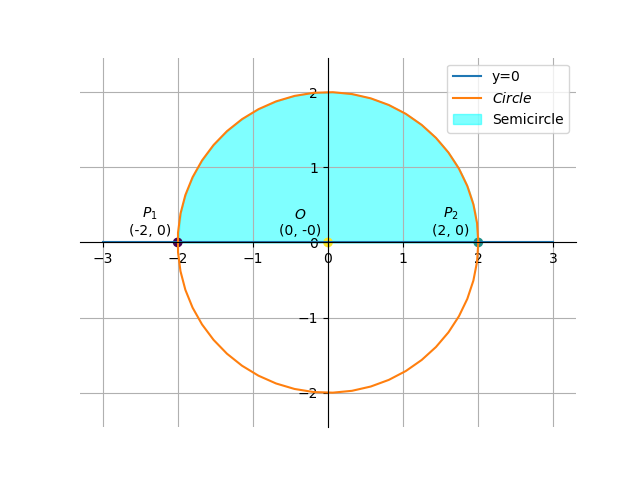
\includegraphics[width=0.7\columnwidth]{plot.png} 
   \caption*{Fig : Circle}
  \label{Fig1}
\end{figure}

\end{document}
